\documentclass{beamer}
\usetheme[secheader]{Madrid} % Themes without Navigation Bars
%\usetheme{PaloAlto} % Themes with a table of contents sidebar
%\usetheme{Copenhagen} % Themes with section and subsection tables

% Manage images
\usepackage{graphicx}
\graphicspath{ {./images/} }

\usepackage[table]{xcolor}

% Custom commands
\newcommand{\highlight}[1]{{\color{blue} #1}}

% Title page and author information
\title{USpekPy Package}
\subtitle{Uncertainty estimation on protection quantities for x-rays using SpekPy and Monte Carlo techniques}
\author[X. Campo]{Xandra Campo}
\institute[LMRI-CIEMAT]{Ionizing Radiation Metrology Laboratory (LMRI) \newline CIEMAT, Spain}
\date{June 2024}

\begin{document}
	\maketitle
	
	\begin{frame}
		\frametitle{Table of Contents}
		\tableofcontents[hideallsubsections]
	\end{frame}
	
	\section{Wellcome to USpekPy!}
	
	\begin{frame}
		\frametitle{Wellcome to USpekPy!}
		\tableofcontents[
		currentsection,
		sectionstyle=show/shaded,
		subsectionstyle=show/show/hide
		]
	\end{frame}
	
	\subsection{What is USpekPy?}
	
	\begin{frame}
		\frametitle{What is USpekPy?}
		\begin{itemize}
			\setlength\itemsep{1em}
			\item \highlight{Python package}: Open source and GPLv3-licensed library compatible with Python 3
			\href{https://github.com/lmri-met/uspekpy}{\beamergotobutton{Go}}
			\item \highlight{Goal}: Compute mean radiation protection quantities for a simulated x-ray spectrum with uncertainties using Monte Carlo techniques
			\item Based on \highlight{SpekPy}: Python package for modelling the x-ray spectra from x-ray tubes
			\href{https://bitbucket.org/spekpy/spekpy_release/wiki/Home}{\beamergotobutton{Go}}
		\end{itemize}
		\bigskip
		\centering
		\href{https://forms.gle/uCHj4XH5BJTBqjiQ9}{\beamergotobutton{Python usage poll}}		
	\end{frame}
	
	\subsection{Main features of USpekPy}
	
	\begin{frame}
		\frametitle{Main features of USpekPy}
		\begin{itemize}
			\setlength\itemsep{1em}
			\item Compute \highlight{mean values of radiation protection quantities} of a simulated x-ray spectrum: $\overline{E}$, $K_{air}$ and $\overline{h_K}$
			\item Compute \highlight{mean radiation protection quantities} of a simulated x-ray spectrum \highlight{with uncertainties} using Monte Carlo techniques: first and second HVL for Al and Cu, $\overline{E}$, $K_{air}$ and $\overline{h_K}$
			\item Perform \highlight{batch simulation} to compute mean values and uncertainties of radiation protection quantities for \highlight{several simulated x-ray spectra}
		\end{itemize}
	\end{frame}
	
	\subsection{USpekPy in a nutshell}
	
	\begin{frame}
		\frametitle{USpekPy in a nutshell}
		\begin{footnotesize}
			\begin{columns}
				\begin{column}{0.32\textwidth}
					\begin{block}{Status}
						\begin{tabular}{ll}
							Last version:&1.0.2\\
							Release date:&Jun 2024\\
							Maintenance:&Active\\
						\end{tabular}
					\end{block}
					\begin{block}{Testing}
						\begin{tabular}{ll}
							Tests:&Passing\\
							Code coverage:&65\%\\
						\end{tabular}
					\end{block}
					\begin{block}{Requirements}
						\begin{tabular}{ll}
							Python:&$\ge$3.8\\
							Dependencies:&spekpy\\
							&pandas\\
							&openpyxl\\
						\end{tabular}
					\end{block}
				\end{column}
				\begin{column}{0.55\textwidth}
					\begin{block}{Links}
						\begin{tabular}{lll}
							Source code:&GitHub&\href{https://github.com/lmri-met/uspekpy}{\beamergotobutton{Go}}\\
							Documentation:&README @GitHub&\href{https://github.com/lmri-met/uspekpy\#README}{\beamergotobutton{Go}}\\
							Contribute:&Issues @GitHub&\href{https://github.com/lmri-met/uspekpy/issues}{\beamergotobutton{Go}}\\
						\end{tabular}
					\end{block}
					\begin{block}{Distribution}
						\begin{tabular}{lll}
							Distribution:&PyPI&\href{https://pypi.org/project/uspekpy/}{\beamergotobutton{Go}}\\
							License:&GNU GPL v3.0&\href{https://github.com/lmri-met/uspekpy?tab=GPL-3.0-1-ov-file}{\beamergotobutton{Go}}\\
						\end{tabular}
					\end{block}
					\begin{block}{Authors}
						\begin{tabular}{ll}
							Authors:&X. Campo \& P. Avilés\\
							Email:&xandra.campo@ciemat.es\\
							&paz.aviles@ciemat.es\\
							Organization:&LMRI-Met @GitHub \href{https://github.com/lmri-met}{\beamergotobutton{Go}}\\
						\end{tabular}
					\end{block}
				\end{column}
			\end{columns}
		\end{footnotesize}
	\end{frame}
	
	\subsection{How to get support?}
	
	\begin{frame}
		\frametitle{How to get support?}
		\begin{columns}[t]
			\begin{column}{0.45\textwidth}
				\begin{block}{\centering Package documentation}
					\centering
					Check the \highlight{documentation} of USpekPy at GitHub
					\href{https://github.com/lmri-met/uspekpy\#readme}{\beamergotobutton{Go}}\\
					\medskip
					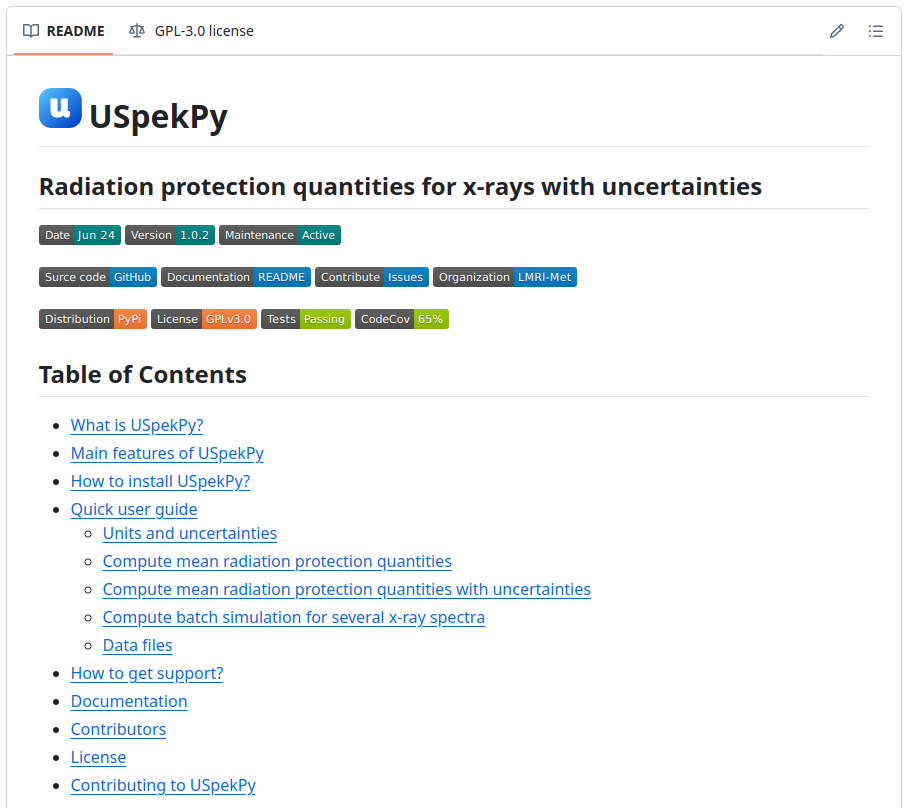
\includegraphics[width=\textwidth]{readme}
				\end{block}
			\end{column}
			\begin{column}{0.45\textwidth}
				\begin{block}{\centering Contact developers}
					\centering
					\bigskip
					Contact the developers of USpekPy \highlight{via email}:\\
					\bigskip
					Xandra Campo\\xandra.campo@ciemat.es\\
					\bigskip
					Paz Avilés\\paz.aviles@ciemat.es
				\end{block}	
			\end{column}
		\end{columns}
	\end{frame}
	
	\subsection{How to contribute to USpekPy?}
	
	\begin{frame}
		\frametitle{How to contribute to USpekPy?}
		\begin{columns}[t]
			\begin{column}{0.45\textwidth}
				\begin{block}{What may be a contribution?}
					\begin{itemize}
						\item Bug reports \& fixes
						\item Documentation improvements
						\item Feature enhancements
					\end{itemize}
				\end{block}
			\end{column}
			\begin{column}{0.45\textwidth}
				\begin{block}{How to deliver a contribution?}
					\begin{itemize}
						\item \highlight{Issues page} at GitHub (Recommended) \href{https://github.com/lmri-met/uspekpy/issues}{\beamergotobutton{Go}}
						\item Contact the developers \highlight{via email}
					\end{itemize}
				\end{block}	
			\end{column}
		\end{columns}
		\bigskip
		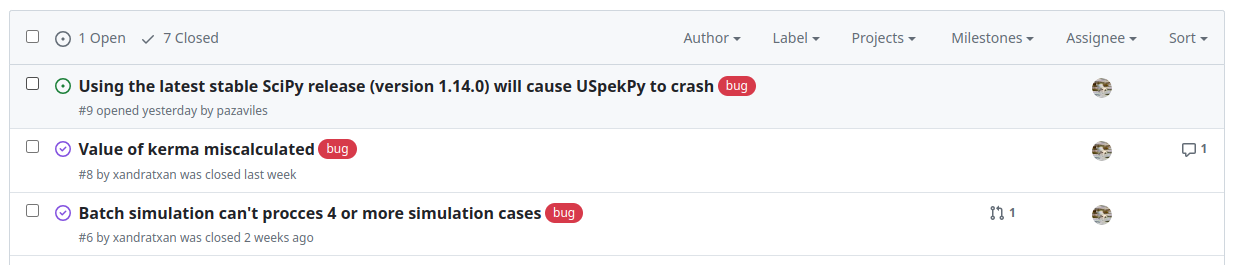
\includegraphics[width=\textwidth]{issues_list}
	\end{frame}
	
	\begin{frame}
		\frametitle{What to include in a contribution?}
		\begin{columns}
			\begin{column}{0.3\textwidth}
				\footnotesize
				\begin{itemize}
					\item Title
					\item Description
					\item Expected behavior
					\item Steps to reproduce
					\item Minimal, reproducible example
					\item Environment
					\item Error messages, logs
					\item Potential fix
				\end{itemize}
			\end{column}
			\begin{column}{0.7\textwidth}
				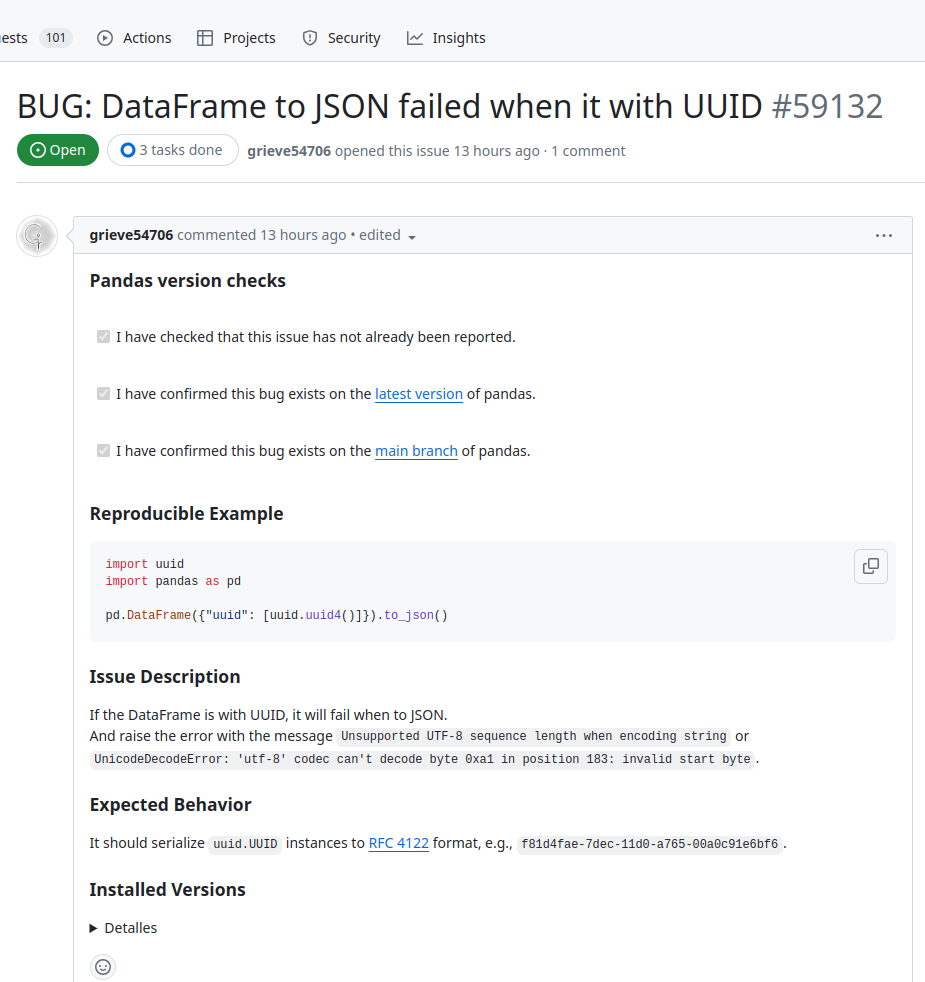
\includegraphics[width=\textwidth]{pandas_issue}
			\end{column}
		\end{columns}
	\end{frame}
	
	\section{How does USpekPy package work?}
	
	\begin{frame}
		\frametitle{How does USpekPy package work?}
		\tableofcontents[
		currentsection,
		sectionstyle=show/shaded,
		subsectionstyle=show/show/hide
		]
	\end{frame}
	
	\subsection{Compute mean radiation protection quantities}
	
	\begin{frame}
		\frametitle{Compute mean radiation protection quantities}
		\framesubtitle{Information flow}
		For a \highlight{single case}, given an x-ray quality and an operational quantity at a specific irradiation angle:
		\begin{columns}[t]
			\begin{column}{0.3\textwidth}
				\begin{block}{Input}
					Value:
					\begin{itemize}
						\item Filter thickness
						\item Peak kilovoltage
						\item Anode angle
						\item $\frac{\mu_{tr}}{\rho}(E)$
						\item $h_K(E)$
					\end{itemize}
				\end{block}
			\end{column}
			\begin{column}{0.3\textwidth}
				\begin{block}{Tool}
					SpekWrapper class
				\end{block}
			\end{column}
			\begin{column}{0.3\textwidth}
				\begin{block}{Output}
					Value:
					\begin{itemize}
						\item HVL(Al, Cu)
						\item $\overline{E}$
						\item $K_{air}$
						\item $\overline{h_K}$
					\end{itemize}
				\end{block}
			\end{column}
		\end{columns}
	\end{frame}
	
	\begin{frame}
		\frametitle{Compute mean radiation protection quantities}
		\framesubtitle{Workflow}
		Workflow for $\overline{E}$, $K_{air}$ and $\overline{h_K}$:
		\begin{columns}
			\begin{column}{0.55\textwidth}
				\begin{enumerate}
					\item Compute x-ray \highlight{spectrum} (energy and fluence) using SpekPy
					\item If necessary, \highlight{interpolate} $\frac{\mu_{tr}}{\rho}(E)$ and $h_K(E)$ to spectrum energies in logarithmic scale
					\item If necessary, apply \highlight{units} conversion
					\item Compute the \highlight{integral quantity} using the corresponding definition
				\end{enumerate}
			\end{column}
			\begin{column}{0.4\textwidth}
				\small
				$$\overline{E}=\frac{\int_{0}^{\infty}\phi(E)EdE}{\int_{0}^{\infty}\phi(E)dE}$$
				$$K_{air}=\int_{0}^{\infty}\phi(E)\frac{\mu_{tr}}{\rho}(E)EdE$$
				$$\overline{h_K}=\frac{\int_{0}^{\infty}\phi(E)\frac{\mu_{tr}}{\rho}(E)h_K(E)EdE}{\int_{0}^{\infty}\phi(E)\frac{\mu_{tr}}{\rho}(E)EdE}$$
			\end{column}
		\end{columns}
		\bigskip
		\highlight{HVLs} are calculated using SpekPy methods.
	\end{frame}
	
	\subsection{Compute mean radiation protection quantities with uncertainties}
	
	\begin{frame}
		\frametitle{Compute mean RP quantities with uncertainties}
		\framesubtitle{Information flow}
		For a \highlight{single case}, given an x-ray quality and an operational quantity at a specific irradiation angle:
		\begin{columns}[t]
			\begin{column}{0.35\textwidth}
				\begin{block}{Input}
					Value and uncertainty:
					\begin{itemize}
						\item Filter thickness
						\item Peak kilovoltage
						\item Anode angle
						\item $\frac{\mu_{tr}}{\rho}(E)$
					\end{itemize}
					Value:
					\begin{itemize}
						\item $h_k(E)$
						\item Number of iterations
					\end{itemize}
				\end{block}
			\end{column}
			\begin{column}{0.23\textwidth}
				\begin{block}{Tool}
					USpek class
				\end{block}
			\end{column}
			\begin{column}{0.32\textwidth}
				\begin{block}{Output}
					Value and uncertainty:
					\begin{itemize}
						\item HVL(Al, Cu)
						\item $\overline{E}$
						\item $K_{air}$
						\item $\overline{h_K}$
					\end{itemize}
				\end{block}
			\end{column}
		\end{columns}
	\end{frame}
	
	\begin{frame}
		\frametitle{Compute mean RP quantities with uncertainties}
		\framesubtitle{Workflow}
		A simulation is performed for the specified number of iterations.
		\bigskip
		\begin{enumerate}
			\setlength\itemsep{1em}
			\item For each iteration:
			\begin{enumerate}
				\item \highlight{Generate random values} of the input variables considering their mean values, uncertainties and distributions.
				\item \highlight{Compute mean values} of the integral quantities using the SpekWrapper class
			\end{enumerate}
			\item Once the iterations are completed:\\
			\highlight{Compute statistical mean value and standard deviation} of the integral quantities from the different values obtained in the iterations
		\end{enumerate}
	\end{frame}
	
	\subsection{Compute batch simulation for several x-ray spectra}
	
	\begin{frame}
		\frametitle{Compute batch simulation for several x-ray spectra}
		\framesubtitle{Information flow}
		For a \highlight{set of cases}, each case for a given x-ray quality and operational quantity at an irradiation angle:
		\begin{footnotesize}
			\begin{columns}[t]
				\begin{column}{0.35\textwidth}
					\begin{block}{Input}
						For every case:\\
						Value and uncertainty:
						\begin{itemize}
							\item Filter thickness
							\item Peak kilovoltage
							\item Anode angle
							\item $\frac{\mu_{tr}}{\rho}(E)$
						\end{itemize}
						Value:
						\begin{itemize}
							\item $h_k(E)$
							\item Number of iterations
						\end{itemize}
					\end{block}
				\end{column}
				\begin{column}{0.23\textwidth}
					\begin{block}{Tool}
						batch\_simulation function
					\end{block}
				\end{column}
				\begin{column}{0.32\textwidth}
					\begin{block}{Output}
						For every case, \\value and uncertainty:
						\begin{itemize}
							\item HVL(Al, Cu)
							\item $\overline{E}$
							\item $K_{air}$
							\item $\overline{h_K}$
						\end{itemize}
					\end{block}
				\end{column}
			\end{columns}
	\end{footnotesize}
	\end{frame}
	
	\begin{frame}
		\frametitle{Compute batch simulation for several x-ray spectra}
		\framesubtitle{Workflow}
		\begin{enumerate}
			\setlength\itemsep{1em}
			\item The set of cases are provided in an \highlight{input file}, each case is a column in that file
			\item For each case, a \highlight{simulation} is performed for the specified number of iterations using the USpek class
			\item Results for the set of cases are returned in an \highlight{output file}, appending the result to the corresponding column of the input file
		\end{enumerate}
	\end{frame}
	
	\subsection{Units and uncertainties convention}
	
	\begin{frame}
		\frametitle{Units and uncertainties convention}
		\begin{itemize}
			%\setlength\itemsep{1em}
			\item All the uncertainties are standard uncertainties (k = 1)
			\item The units of relative uncertainties are expressed as fraction of one
		\end{itemize}
		\bigskip
		\centering
		\rowcolors{2}{gray!15}{white}
		\begin{tabular}{cc}
			\rowcolor{blue!25}
			\textbf{Quantity}&\textbf{Unit}\\
			Distance&mm\\
			Voltage&kV\\
			Angle&deg\\
			Energy&keV\\
			Fluence&1/cm²\\
			Mass energy transfer coefficients of air&cm²/g\\
			Air kerma&uGy\\
			Mono-energetic K to H conversion coefficients&Sv/Gy\\
		\end{tabular}
	\end{frame}
	
	\subsection{Verification of the code}
	
	\begin{frame}
		\frametitle{Verification of the code}
		\begin{itemize}
			\setlength\itemsep{2em}
			\item Integral quantity \highlight{values}: Compared with values provided by SpekPy (except $\overline{h_K}$)
			\item Integral quantity \highlight{uncertainties}: Compared with values provided by:
			\begin{itemize}
				\setlength\itemsep{1em}
				\item Previous script version of USpekPy developed by Paz Avilés
				\item Results obtained by CMI
			\end{itemize}
		\end{itemize}
	\end{frame}
	
	\section{How to use USpekPy?}
	
	\begin{frame}
		\frametitle{How to use USpekPy?}
		\tableofcontents[
		currentsection,
		sectionstyle=show/shaded,
		subsectionstyle=show/show/hide
		]
	\end{frame}
	
	\section{Wrapping up: What’s next?}
		
	\begin{frame}
		\frametitle{Wrapping up: What’s next?}
		\tableofcontents[
		currentsection,
		sectionstyle=show/shaded,
		subsectionstyle=show/show/hide
		]
	\end{frame}
	
	\subsection{Improvements on the horizon}
	
	\begin{frame}
		\frametitle{Improvements on the horizon}
		\begin{itemize}
			\setlength\itemsep{1em}
			\item \highlight{Bug}: Fix SciPy dependency bug
			\item \highlight{New feature}: Add the contribution to the \highlight{uncertainty} of the variation of the mono-energetic air kerma-to-dose conversion coefficients
			\item \highlight{Documentation}: Improve package documentation (GitHub Wiki, GitHub Pages)
			\item \highlight{Testing}: Improve test code coverage
		\end{itemize}			
	\end{frame}
	
	\subsection{Let us know what you think}
	
	\begin{frame}
		\frametitle{Let us know what you think}
		\centering
		\highlight{Complete our satisfaction survey about this seminar!}
		
		Help us make future seminars better.
		
		\bigskip
		
		\href{https://forms.gle/zymzqsLidy5uxKQV6}{\beamergotobutton{Satisfaction survey}}
		
		\bigskip
		
		\highlight{Contribute to USpekPy package!}
		
		This sofware is for you. We want to make it fit better your necesities. Let us know if you find any issue or if you would like to have any new feature in future versions.
		
		\bigskip
		
		\href{https://github.com/lmri-met/uspekpy/issues}{\beamergotobutton{USpekPy Issues page}}
		
		xandra.campo@ciemat.es
		
		paz.aviles@ciemat.es
	\end{frame}
	
	\begin{frame}
		\frametitle{Thank you very much!}
		\centering
		We’re grateful for your time and attention today. 
		
		We appreciate your interest in USpekPy.
		
		Thank you for joining us.
	\end{frame}
	
\end{document}
